\chapter{Measuring Team Progress and Adaptation}
\label{ch:agile-evaluation}

Adopting Agile is only the beginning. Teams must continuously evaluate whether their implementation delivers value and identify areas for improvement. Empiricism requires inspection and adaptation based on transparent information \textit{\parencite{schwaber2020scrum}}. Research shows that teams demonstrating responsiveness through frequent releases achieve higher stakeholder satisfaction \textit{(Russo, ASE Lecture 3, 2025)}. This chapter examines how Djøf Trade Union measures their Agile effectiveness and evolves their practices.

\section{Sprint Reviews and Stakeholder Engagement}
\label{sec:sprint-reviews}

Djøf Trade Union established regular sprint reviews to evaluate completed work and gather feedback. After each sprint, they review accomplishments, whether goals were met, and lessons learned \textbf{(Transcript: 00:06:48)}. These reviews provide structured moments for reflection rather than pushing forward blindly.

Reviews involve business stakeholders. The team invites interested parties to see what they built, and quarterly demos showcase accumulated progress to broader audiences \textbf{(Transcript: 00:20:37)}. This demonstration rhythm keeps stakeholders informed without constant interruptions.

The review process helps understand whether work delivers actual value. When features reach users, the Product Owner collects feedback and brings it back to development \textbf{(Transcript: 00:21:07)}. This creates a feedback loop where user experience influences prioritization. Success means solving real problems for members and internal users, not just completing tasks.

\section{Retrospectives and Process Refinement}
\label{sec:retrospectives}

Beyond reviewing product increments, the team holds retrospectives to examine working methods. These sessions focus on collaboration and obstacles \textbf{(Transcript: 00:07:31)}. Sprint Retrospectives enable teams to reflect on process and identify improvements \textit{(Russo, ASE Lecture 3, 2025)}.

One concrete improvement emerged from discussions: code reviews took too long because colleagues lacked time for prompt examination \textbf{(Transcript: 00:23:07)}. The team agreed that when someone creates a pull request and announces it in Teams, a reviewer must examine it within four hours \textbf{(Transcript: 00:23:37)}. This commitment dramatically improved development flow.

The team's pragmatic adaptation appears in retrospectives too. When sprints lack meaningful progress, they skip the retrospective because there is little to reflect upon \textbf{(Transcript: 00:09:59)}. This demonstrates focus on value rather than ceremony.

\section{Tracking Metrics and Leadership Support}
\label{sec:tracking-metrics}

Djøf Trade Union tracks concrete indicators of progress. They measure tasks completed per sprint for capacity insight \textbf{(Transcript: 00:21:52)} and lead time from task start to production deployment, highlighting bottlenecks.

Quality metrics complement velocity tracking. The team monitors bugs during development versus those escaping to production \textbf{(Transcript: 00:22:22)}. This indicates whether testing catches issues before users encounter them. Quality assurance practices and Definition of Done criteria help maintain standards \textit{(Russo, ASE Lecture 5, 2025)}. High production bug rates signal problems with testing or code review.

Their measurement approach remains practical rather than exhaustive. They gather enough data to spot trends without drowning in metrics. The goal is actionable insight. When code review delays appeared in data and discussions, they took concrete action rather than documenting the problem.

\begin{figure}[h]
\centering
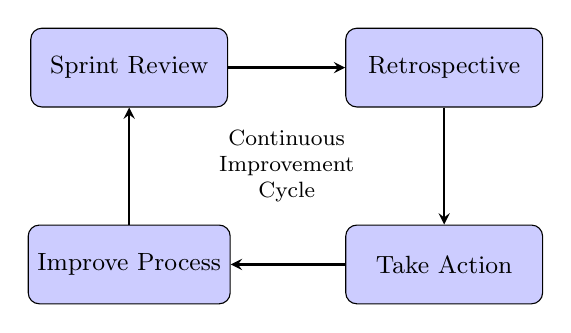
\begin{tikzpicture}
    % Define styles
    \tikzstyle{process} = [rectangle, rounded corners, minimum width=2.5cm, minimum height=1cm,
                          text centered, draw=black, fill=blue!20, font=\small]
    \tikzstyle{arrow} = [thick,->,>=stealth]

    % Nodes positioned absolutely
    \node[process] (review) at (0,0) {Sprint Review};
    \node[process] (retro) at (4,0) {Retrospective};
    \node[process] (action) at (4,-2.5) {Take Action};
    \node[process] (improve) at (0,-2.5) {Improve Process};

    % Arrows
    \draw[arrow] (review) -- (retro);
    \draw[arrow] (retro) -- (action);
    \draw[arrow] (action) -- (improve);
    \draw[arrow] (improve) -- (review);

    % Center label
    \node[font=\footnotesize, text width=2cm, align=center] at (2,-1.25) {Continuous\\Improvement\\Cycle};
\end{tikzpicture}
\caption{Continuous improvement cycle through regular sprint reviews and retrospectives}
\label{fig:improvement-cycle}
\end{figure}


Sprint reviews, retrospectives, and lightweight metrics create continuous improvement. The organization demonstrates that Agile evaluation requires neither sophisticated tools nor extensive data collection. Regular inspection of product and process, coupled with willingness to adapt when issues surface, drives improvement.

Management support reinforces this learning orientation \textbf{(Transcript: 00:24:22)}, allowing investment in addressing problems rather than only delivering features. Leadership provides resources for skill development and respects process boundaries. This creates psychological safety where teams acknowledge problems without fear, enabling honest retrospectives.
